\documentclass[conference,letterpaper]{IEEEtran}
\usepackage[T1]{fontenc}
\usepackage{amsmath,amssymb}
\usepackage{booktabs}
\usepackage{tikz}
\usetikzlibrary{arrows.meta,positioning}
\usepackage{balance}
\usepackage[hidelinks]{hyperref}
\hypersetup{pdftitle={Policy-Consistent Federated Learning: Dynamic Governance and Auditable Aggregation},pdfauthor={Muzakkiruddin Ahmed Mohammed; Sana Afsheen Shaik; Alyson Michele Chapman; Abdelrahman Elfikky; John Talburt}}
\newcommand{\method}{P1}
\begin{document}
\title{Policy-Consistent Federated Learning:\\Dynamic Governance and Auditable Aggregation}
\author{
\IEEEauthorblockN{Muzakkiruddin Ahmed Mohammed\textsuperscript{*}, Sana Afsheen Shaik\textsuperscript{\textasciicircum}, Alyson Michele Chapman\textsuperscript{\textasciicircum},\\
Abdelrahman Elfikky\textsuperscript{*}, and John Talburt\textsuperscript{*}}
\IEEEauthorblockA{\textsuperscript{*}Center for Advanced Research in Entity Resolution and Information Quality (ERIQ)\\
University of Arkansas at Little Rock\\
\textsuperscript{\textasciicircum}Bentonville West High School\\
mmohammed6@ualr.edu, shaiks@bentonvillek12.org, chapmanal@bentonvillek12.org\\
aelfikky1@ualr.edu, Jrtalburt@ualr.edu}}
\maketitle

\begin{abstract}
Federated learning separates local computation from aggregation, but an update authorized at dispatch may become ineligible before publication. We evaluate a policy-consistent protocol that checks inclusive authorization histories and guards the transition to a published model. Eight separately authenticated clients use a policy authority, versioned object storage, transactional publication state and independently protected audit evidence. A fixed primary benchmark crosses four methods, two data distributions, four scenarios and five training seeds. The proposed protocol incorporated zero of 20 oracle-invalid presented updates, compared with 20 of 20 for dispatch-only authorization. Under stable policies, paired test-AUROC differences were zero; ratios of mean round times indicated 3.3\% and 18.5\% overhead under IID and non-IID partitions, respectively. Audit evidence was complete in the observed inclusion scope, but the registered runtime-manipulation hypothesis remained inconclusive. These results support an incremental protocol evaluation under explicit trust assumptions, rather than population-level safety or clinical effectiveness.
\end{abstract}
\begin{IEEEkeywords}
federated learning, dynamic authorization, data governance, auditable aggregation, transactional publication
\end{IEEEkeywords}

\section{Introduction and Related Work}
Federated averaging (FedAvg) combines locally trained models without requiring a pooled training table~\cite{fedavg}. This separation does not determine whether a contribution remains authorized when collaboration policies change. An organization can be revoked after dispatch, or lose and regain permission while an update is in flight. A check immediately before aggregation can also race a policy mutation before the resulting model is published. These are temporal authorization problems, even when training and communication follow their specifications.

Continuous authorization and mutable attributes are established usage-control concepts~\cite{ucon}. Policy-aware FL is also prior art: AspectFL integrates policies and provenance~\cite{aspectfl}; policy-driven FL describes lifecycle enforcement and observability~\cite{pdfl}; and PoCoFL studies policy compliance using commitments and zero-knowledge proofs~\cite{pocofl}. Our comparison with policy-driven FL is limited to its abstract: its precise interruption and publication semantics remain unknown. We make no firstness claim or performance comparison with these systems.

Our contribution is a concrete, history-aware publication protocol and a controlled deployment evaluation. We ask whether an update remains eligible throughout its lifecycle, whether publication can preserve that decision despite concurrent policy changes, and what the checks cost in model utility and runtime. The study distinguishes preventing an invalid contribution from retaining evidence that a decision occurred.

\section{History-Aware Model Publication}
\subsection{Eligibility and Trust Boundary}
Eight fictional organizations each run a separately authenticated client. Tasks and updates bind organization, purpose, round, nonce, schema and content digest. Policies use exact purpose strings and three actions: \texttt{train}, \texttt{submit\_update} and \texttt{aggregate}. Denials override allowances, and missing permission denies. Each authority mutation atomically appends immutable history and advances the organization's contiguous epoch.

For update $u$ from organization $o$, let $\mathcal{H}_o[u]$ contain the policy state at task acknowledgment and every subsequent authority transition through publication. Eligibility requires
\begin{equation}
 E(u)=\bigwedge_{h\in\mathcal{H}_o[u]}\ \bigwedge_{a\in\mathcal{A}}
 \operatorname{Allow}(h,o,p_u,a),
 \label{eq:eligibility}
\end{equation}
where $\mathcal{A}$ is the three-action set and $p_u$ is the bound purpose. A relevant denial permanently invalidates that task lifecycle, including after regrant. An unrelated-purpose mutation can preserve eligibility but requires epoch revalidation. Missing history, inconsistent tails or incomplete pagination fail closed. Expiry is an explicit authority transition; the protocol supplies no hard wall-clock expiry guarantee or retroactive removal from previously committed models.

The design trusts identity mapping, policy writers, enforcement and order services, durable staged objects and separately protected audit anchors. Clients are not thereby proven to train truthfully. Differential privacy, secure aggregation, poisoning resistance and unlearning are outside the evaluation.

\subsection{Guarded Commit and Independent Checking}
The coordinator checks authorization at dispatch and receipt, then reads a coherent authority snapshot and complete history prefixes. Eligible updates form a sample-weighted FedAvg candidate using unique contributing sample counts. Before publication, the system stages the candidate in versioned S3 storage and verifies its exact version, digest, size and availability (Fig.~\ref{fig:protocol}).

\begin{figure}[t]
\centering
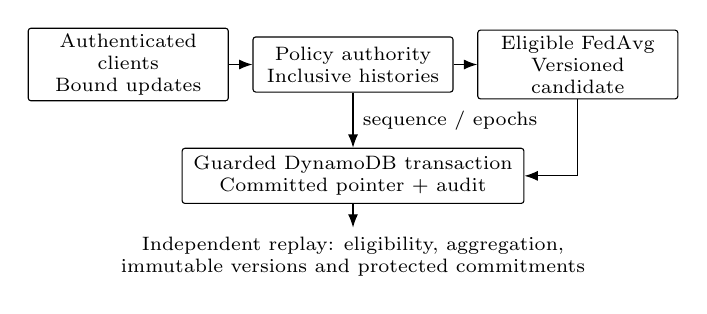
\begin{tikzpicture}[font=\scriptsize,box/.style={draw,rounded corners=1pt,align=center,inner sep=2pt,minimum height=7mm,text width=24mm},>=Latex]
\node[box] (clients) {Authenticated clients\\Bound updates};
\node[box,right=3mm of clients] (history) {Policy authority\\Inclusive histories};
\node[box,right=3mm of history] (candidate) {Eligible FedAvg\\Versioned candidate};
\node[box,below=7mm of history,text width=42mm] (commit) {Guarded DynamoDB transaction\\Committed pointer + audit};
\draw[->] (clients) -- (history);
\draw[->] (history) -- (candidate);
\draw[->] (candidate.south) |- (commit.east);
\draw[->] (history) -- node[right]{sequence / epochs} (commit);
\node[below=3mm of commit,align=center] (verify) {Independent replay: eligibility, aggregation,\\immutable versions and protected commitments};
\draw[->] (commit) -- (verify);
\end{tikzpicture}
\caption{Publication binds a verified staged object to a guarded pointer transition. The object store and transaction service are separate; publication linearizes at the committed pointer.}
\label{fig:protocol}
\end{figure}

A single DynamoDB transaction guards the global authority sequence, contributor epochs, parent-model pointer, round-membership generation, pending-update finality and audit state. It records the manifest, final outcomes and audit updates while advancing the committed pointer. This transition is the release linearization point; S3 and DynamoDB do not form a cross-service atomic transaction. Conflicts require refreshed history, membership and aggregation. Durable operation fingerprints resolve ambiguous responses, while unique update identities prevent duplicate contribution.

Under the stated assumptions, a relevant mutation before commit changes a guarded authority value and prevents stale publication. A mutation ordered after commit does not retroactively invalidate the earlier model. This reasoning depends on complete history and controlled writers, not merely on the presence of an audit log. Independent checks reconstruct eligibility, weighted aggregation, object versions, audit membership and pointer consistency. Separately retained operator commitments and an externally bound signing-key fingerprint protect the reference point; tamper evidence depends on that custody, as in prior logging work~\cite{logging}.

\section{Experimental Design}
The historical UCI Diabetes 130-US Hospitals benchmark~\cite{uci} contains 101,766 encounters from 71,518 patients. A patient-grouped 70/15/15 split yields 71,160 training, 15,324 validation and 15,282 test encounters. The binary target is readmission within 30 days. Preprocessing is fitted on training data only and produces 194 features. Patient identifiers and declared outcome-proxy fields are excluded from predictors.

Eight fictional clients receive balanced IID allocation or label-stratified Dirichlet allocation with concentration $\alpha=0.5$, keeping patient groups intact. A float32 CPU multilayer perceptron has 64- and 32-unit ReLU hidden layers. Each of five global rounds uses one local epoch, Adam with learning rate 0.001 and batches of 64. Deployment uses AWS Fargate, Open Policy Agent, DynamoDB and versioned S3 in one account and region. The distributions share the same cohort and represent simulated organizations rather than actual hospital partitions.

The fixed primary matrix contains $4\times2\times4\times5=160$ cells. Methods are B1 (policy ignored, structural/custody checks retained), B2 (initial organization admission cached), B3 (dispatch authorization cached) and \method{} (dispatch, receipt, inclusive history and guarded commit). Scenarios are S0 (stable), S1 (between-round revocation), S2 (in-flight revocation) and S3 (revocation with delayed update delivery). Matched methods share data, initialization, training and intervention bindings. Five seeds are 296, 593, 887, 1181 and 1483.

An independent oracle reconstructs eligibility from retained authority events. H1 tests for P1 invalid incorporation; H2 compares invalid-incorporation rates against B2 and B3; H3 requires complete audit evidence and runtime-manipulation detection with successful targeted coverage; H4 tests stable-policy AUROC noninferiority against B3.

Inference resamples five paired training-seed clusters, conditional on the fixed cohort and client setup. The 160 cells and individual updates are not independent replicates. Paired percentile bootstrap intervals use 10,000 resamples and RNG seed 271828. Invalid incorporation divides invalid incorporated updates by oracle-invalid presented updates; incorrect rejection uses oracle-valid presented updates. Zero-opportunity ratios remain undefined. H2 pools S1--S3 and both distributions within seed; H4 uses only S0 P1/B3 pairs, with a prespecified AUROC margin of $-0.02$.

\section{Results and Limitations}
\subsection{Authorization, Utility and Overhead}
All 160 primary cells completed successfully. Table~\ref{tab:governance} reports observed governance outcomes. P1 incorporated 0/20 oracle-invalid presented updates; B3 incorporated 20/20. B1 and B2 each incorporated 140/140, reflecting different presentation opportunities. Each method rejected 0/1460 valid presented updates. These are conditional opportunity counts, not a common-exposure causal comparison.

\begin{table}[t]
\caption{Primary governance counts across both distributions and S0--S3. Opportunity denominators differ by method.}
\label{tab:governance}
\centering
\begin{tabular}{lrr}
\toprule
Method & Invalid incorporated/ & Valid rejected/\\
       & invalid presented & valid presented\\
\midrule
B1: policy ignored & 140/140 & 0/1460\\
B2: admission cached & 140/140 & 0/1460\\
B3: dispatch cached & 20/20 & 0/1460\\
P1: history + commit & 0/20 & 0/1460\\
\bottomrule
\end{tabular}
\end{table}

The registered H1 criterion was met, but zero violating clusters among five seeds yields a conditional one-sided 95\% upper bound of $1-0.05^{1/5}=45.07\%$ for a violating seed cluster. It does not establish zero population risk. For H2, P1-minus-B2 and P1-minus-B3 invalid-incorporation-rate differences were both $-1$, with unadjusted two-sided 95\% intervals $[-1,-1]$. The degenerate intervals reflect identical observed seed-level differences in this finite suite.

Under S0, P1-minus-B3 test-AUROC differences were zero for every matched seed in each distribution. Both one-sided 95\% lower bounds were 0, exceeding the $-0.02$ margin. This meets H4 within the frozen benchmark, without establishing population equivalence or clinical noninferiority. Runtime increased (Table~\ref{tab:runtime}); these observations do not support a negligible-overhead claim. Paired mean-difference 95\% intervals were [0.814, 2.520] seconds under IID and [9.201, 10.690] seconds under non-IID. These describe the fixed primary S0 executions; later support-startup measurements are not substituted into that comparison.

\begin{table}[t]
\caption{Stable S0 P1 versus B3; five paired seeds per distribution. Ratios divide mean round times, not per-seed ratios.}
\label{tab:runtime}
\centering
\begin{tabular}{lrr}
\toprule
Distribution & P1/B3 time ratio & Mean difference (s)\\
\midrule
IID & 1.03344 & 1.612\\
Non-IID & 1.18485 & 10.093\\
\bottomrule
\end{tabular}
\end{table}

\subsection{Evidence Coverage and Qualifications}
The full canonical registry contains 258 attempted obligations: 160 primary, 50 targeted, 40 ablation and eight fresh-replication cells. The unchanged project analysis recorded 248 successful statuses and retained ten targeted failures. All 40 ablations have component-specific partial-protocol verification; the 20 non-IID ablations additionally lack complete five-round evidence. They are not full-P1 safety evidence. Eight replicas used one new deployment and two disjoint client fleets at an existing seed, rather than new independent seed clusters. Twenty-one separate exploratory cases remain single-seed, validation-only descriptions.

\balance
Targeted S4--S7 cover revoke--regrant, expiry, mutation near publication, and duplicate/reordered consumption with restart. Each scenario completed five cells per distribution (40 successes). All ten S8 transport-fault cells failed and remain in the registered coverage denominator. A scheduled intervention alone is not evidence that its intended runtime behavior occurred; retained traces and verifier scope govern interpretation.

Component ablations help distinguish the mechanisms. Replacing continuous history with current-state authorization (Abl-4) admitted 5/5 invalid presented updates in each distribution, consistent with the revoke--regrant gap. Removing receipt rechecking (Abl-1) or contributor-epoch conditions (Abl-2) yielded 0/5 in each distribution. Abl-2 still retains the global sequence fence, so its result does not establish that publication guards can be discarded. Omitting final-decision audit appends (Abl-3) yielded 0/200 complete audited decisions per distribution; its invalid-presentation denominator was zero and its invalid-incorporation rate remains undefined. These are descriptive component checks with five registered seeds per condition, under the partial-verification qualifications above.

Under the fixed non-ablated P1 inclusion rules, audit completeness was 3304/3304 final decisions and verification covered 94/94 record sets. Nevertheless, H3 remained inconclusive: runtime manipulation detection was undefined (0/0; no attempted runtime manipulations) and only 40/50 targeted cells succeeded. Six detected manipulations of copied evidence were a separate post-run exercise and do not fill that runtime denominator. Protected replay checked both original runtime images; recomputation of all 269 originally reported final utility outputs passed the fixed comparison policy (exact discrete fields and $10^{-6}$ absolute tolerance for six floating metrics). This is retained-snapshot verification, not remote attestation.

The main limits are five seeds on one fixed historical cohort, simulated organizations and a single-region deployment. Interim validation and held-out metric exposures occurred; settings and analysis were not retuned and favorable retries did not replace failures. The complete record retains those deviations and missing evidence. The independent public-data study does not establish clinical effectiveness, general legal compliance or safety against compromised trusted administrators. Stronger claims require broader cohorts, additional deployments and successful runtime-attack coverage.

\section{Conclusion}
Inclusive authorization history and a guarded publication boundary prevented the observed invalid incorporations in this controlled benchmark while preserving stable-policy AUROC. Measured overhead varied by partition, and runtime-manipulation evidence remained insufficient. The protocol offers an explicit, auditable treatment of lifecycle interruptions and publication races under declared trust assumptions.

\begin{thebibliography}{7}
\bibitem{fedavg} B. McMahan, E. Moore, D. Ramage, S. Hampson, and B. Aguera y Arcas, ``Communication-efficient learning of deep networks from decentralized data,'' in \emph{Proc. AISTATS}, PMLR, vol. 54, 2017, pp. 1273--1282.
\bibitem{ucon} R. Sandhu and J. Park, ``Usage control: A vision for next generation access control,'' in \emph{Computer Network Security (MMM-ACNS)}, LNCS, vol. 2776, 2003, pp. 17--31, doi: 10.1007/978-3-540-45215-7\_2.
\bibitem{aspectfl} A. AlSobeh, A. Shatnawi, and A. Magableh, ``AspectFL: Aspect-oriented programming for trustworthy and compliant federated learning systems,'' \emph{Information}, vol. 16, no. 12, Art. no. 1048, 2025, doi: 10.3390/info16121048.
\bibitem{pdfl} T. Ranathunga, S. Bharti, and A. McGibney, ``Policy-driven federated learning: Operationalising governance, trust, and compliance in cross-organisational AI,'' in \emph{Proc. IEEE SMARTCOMP Companion}, 2026, pp. 141--146, doi: 10.1109/SmartComp-Companion70724.2026.00041. Abstract-only comparison.
\bibitem{pocofl} D. R. George, V. Mishra, and A. Abidin, ``PoCoFL: POlicy-COmpliant Federated Learning,'' arXiv:2610.03650v1, 2026. [Online]. Available: \url{https://arxiv.org/abs/2610.03650v1}
\bibitem{logging} S. A. Crosby and D. S. Wallach, ``Efficient data structures for tamper-evident logging,'' in \emph{Proc. USENIX Security Symp.}, 2009, pp. 317--334.
\bibitem{uci} J. Clore, K. Cios, J. DeShazo, and B. Strack, ``Diabetes 130-US Hospitals for Years 1999--2008,'' UCI Machine Learning Repository, 2014, doi: 10.24432/C5230J.
\end{thebibliography}
\smallskip
\end{document}
